\section{Nichtlineare Optimierung}
\subsection{Definitionen}
  Gradient: $\overline{\grad} f = \nabla f = [f_{x_1}, f_{x_2}, \ldots, f_{x_n} ]^T$ (Spaltenvektor)
  
  Satz von Schwarz: $\frac{\partial^2 f(x_1, x_2)}{\partial x_1 \partial x_2} = \frac{\partial^2 f(x_1, x_2)}{\partial x_2 \partial x_1}$

\subsection{Gradientenverfahren}
  \begin{minipage}{14cm}
    Von der Stelle $\vec{x}^{(i)}$ wird in Richtung des Antigradienten geschritten. 
    $$\vec{x}^{(i+1)} = \vec{x}^{(i)} - \alpha_i \nabla f(\vec{x}^{(i)})$$
    
    Vorteile:
    \begin{liste}
      \item Einfach zu implementieren
      \item Findet optimale Lösung
      \item Keine gute Startnäherung nötig
    \end{liste}
    
    Nachteile:
    \begin{liste}
      \item Konvergiert langsam
      \item In der Nähe der optimalen Lösung Zick-Zack-Kurs
    \end{liste}
  \end{minipage}
  \begin{minipage}{5cm}
    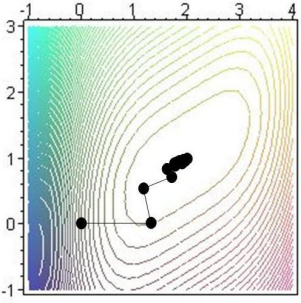
\includegraphics[width=5cm]{./Content/NonLinearOptimization/gradient-descent}
  \end{minipage}
  
  Matlab-Code für das Verfahren (nur ein Loop):
  \begin{MatlabCode}
    % Find betas
    beta1 = 0;
    beta3 = 2; % will be divided by 2 in the loop -> start value = 1
    h_beta1 = subs(f, x, p);
    h_beta3 = 2*h_beta1; % must be higher than h_beta1 (initial)
    while h_beta1 <= h_beta3;
        beta3 = beta3 / 2;
        h_beta3 = subs(f, x, p - beta3 * gradf_numeric);
    end;
    beta2 = beta3/2;
    h_beta2 = subs(f, x, p - beta2 * gradf_numeric);

    % Parabola
    C = h_beta1;
    A = (h_beta3-2.0*h_beta2+C)/(2*beta2*beta2);
    B = (h_beta2-C)/beta2 - beta2*A;
 
    % Candidates for a
    a1 = -B / (2*A);
    a2 = beta3;
    
    % Select a
    if subs(f, x, p - beta3*gradf_numeric) <= h_beta3 
        a = a1;
    else
        a = a2;
    end
    
    
    % Calculate next step
    p = p - a * gradf_numeric;
  \end{MatlabCode}
  
\subsection{Newton-Verfahren}
  \begin{minipage}{14cm}
    Anstelle des Gradienten wird eine Tangente an den Arbeitspunkt gelegt.
    $$\vec{x}^{(i+1)} = \vec{x}^{(i)} - (\bm H(\vec{x}^{(i)}))^{-1} \nabla f(\vec{x}^{(i)})$$
    mit der Hesse-Matrix
    $$\bm{H}(\vec{x})=
    \left(\frac{\partial^2f}{\partial x_i\partial x_j}(x)\right)_{i,j=1,\dots, n}=
    \begin{pmatrix}
    \frac{\partial^2 f}{\partial x_1\partial x_1}(x)&\frac{\partial^2 f}{\partial x_1\partial x_2}(x)&\cdots&\frac{\partial^2  f}{\partial x_1\partial x_n}(x)\\[0.5em]
    \frac{\partial^2 f}{\partial x_2\partial x_1}(x)&\frac{\partial^2 f}{\partial x_2\partial x_2}(x)&\cdots&\frac{\partial^2  f}{\partial x_2\partial x_n}(x)\\
    \vdots&\vdots&\ddots&\vdots\\
    \frac{\partial^2 f}{\partial x_n\partial x_1}(x)&\frac{\partial^2 f}{\partial x_n\partial x_2}(x)&\cdots&\frac{\partial^2  f}{\partial x_n\partial x_n}(x)
    \end{pmatrix}$$
    
    Vorteile:
    \begin{liste}
      \item Gutes Konvergenzverhalten
    \end{liste}
    
    Nachteile:
    \begin{liste}
      \item Hesse-Matrix benötigt zweite Ableitung (numerisch aufwendig)
      \item Inversion der Matrix skaliert schlecht ($O(n^3)$)
    \end{liste}
  \end{minipage}
  \begin{minipage}{5cm}
    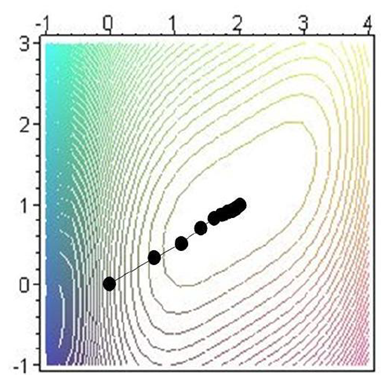
\includegraphics[width=5cm]{./Content/NonLinearOptimization/newton}
  \end{minipage}
  
  
\subsection{Quasi-Newton-Verfahren}
  Um die Berechnung der Ableitungen zu umgehen, werden diese durch finite Differenzen approximiert. 
  
  $$\frac{\partial^2 f}{\partial x_i^2} = \frac{1}{\epsilon^2} 
  \left( f(x_1, x_2, \ldots, x_i+\epsilon, \ldots, x_n) - 2 f(x_1, x_2, \ldots, x_i, \ldots, x_n) + f(x_1, x_2, \ldots, x_i-\epsilon, \ldots, x_n) \right)$$
  
  $$\frac{\partial^2 f}{\partial x_i \partial x_j} = \frac{1}{4 \epsilon^2} \begin{pmatrix}
    f(x_1, x_2, \ldots, x_i+\epsilon, \ldots, x_k+\epsilon, \ldots, x_n) - f(x_1, x_2, \ldots, x_i-\epsilon, \ldots, x_k+\epsilon, \ldots, x_n)\\
    -f(x_1, x_2, \ldots, x_i+\epsilon, , \ldots x_k-\epsilon, \ldots, x_n) + f(x_1, x_2, \ldots, x_i-\epsilon, \ldots, x_k-\epsilon, \ldots, x_n)
  \end{pmatrix}$$